\documentclass[11pt]{article}

%%%%%%%%%%%%%%Include Packages%%%%%%%%%%%%%%%%%%%%%%%%%%
\usepackage{xcolor}
\usepackage{mathtools}
\usepackage[a4paper, total={6in, 8in}, margin=1.25in]{geometry}
\usepackage{amsmath}
\usepackage{amssymb}
\usepackage{paralist}
\usepackage{rsfso}
\usepackage{amsthm}
\usepackage{wasysym}
\usepackage[inline]{enumitem}   
\usepackage{hyperref}
\usepackage{tocloft}
\usepackage{titlesec}
\usepackage{colortbl}
%%%%%%%%%%%%%%%%%%%%%%%%%%%%%%%%%%%%%%%%%%%%%%%%%%%%%%%%



\begin{document}
\Large \noindent \textbf{Physics 5C Discussion (Week 5)}\\
\normalsize
Department of Physics and Astronomy, UCLA\\
%\noindent TA: Jinyan Miao (jnmiu@ucla.edu)\\
%Office hours: Thursday 10-11 AM $\&$ 1-2 PM at PAB 2-429\\
%Tutoring center hours: Friday 2-3 PM at PAB 2-429 (Zoom room also available)\\
\noindent\rule{8cm}{0.4pt}\\
We have studied the electric field in a parallel-plate capacitor in week 3. 
\begin{center}
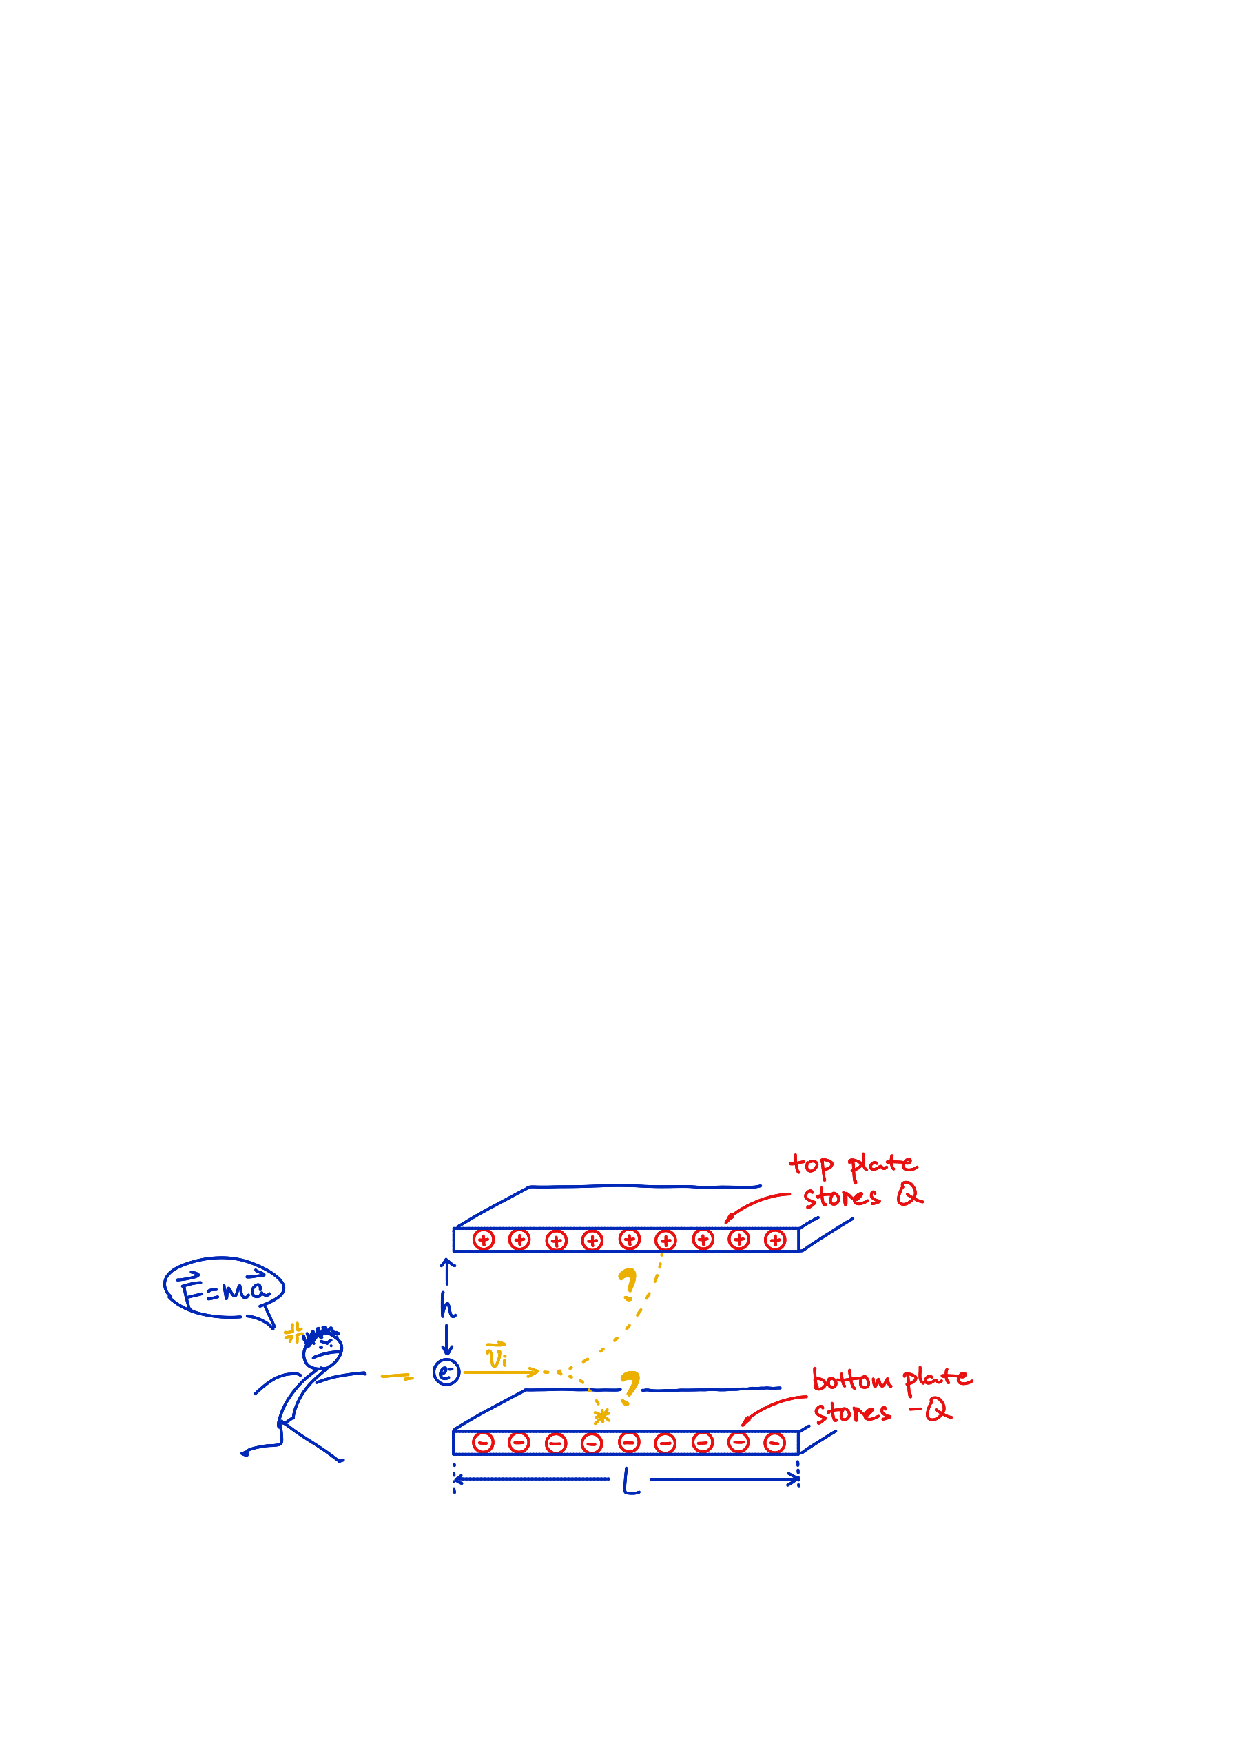
\includegraphics[scale=0.85]{capacitor}
\end{center}
The capacitor is formed by two conducting plates that carry charges as shown. The strength of the electric field between the plates is uniformly given by 
$
|\vec{E}| = Q/(\epsilon_0 A)\,,
$
with $A$ being the area of each of the plates and $Q$ being the amount of positive charges stored at the top plate. There is an equal amount of negative charges $-Q$ stored at the bottom plate. The electric field and potential that we study in the week-4 worksheet problem 2 is in fact the one created by a capacitor. From there, you see that the top and bottom plates have different electric potential, that we call a potential difference $\Delta V$, between the two plates.\\


\noindent \textbf{Part (a)} For a parallel-plate capacitor separated by a distance $d$, show that \footnote{To derive this, you need to combine the $|\vec{E}|=Q/(\epsilon_0 A)$ of a parallel-plate capacitor with what you have learned in the week-4 worksheet problem 2.}
$$\Delta V = \frac{Qd}{\epsilon_0 A}\,.\\$$

In practice, a capacitor is used to store energy. To practically build a capacitor, we connect it to a battery: Starting from two neutral plates separated by some distance $d$, a battery will drive some electrons on one of the plates to move to the other plate via the circuit wires. In this process, some energy from the battery is now transferred to the capacitor. To quantify how much energy is transferred (then stored in the capacitor), we first define the capacitance $C$ of a capacitor,
\begin{align*}
C = \frac{Q}{\Delta V}\,, \qquad \text{measured in Farad (F)}. 
\end{align*}
Then the energy stored in a charged capacitor is
\begin{align*}
U_c = \frac{1}{2}C(\Delta V)^2\,,\qquad \text{measured in Jouls (J)}.
\end{align*}
\noindent \textbf{Part (b)} Using part (a), for the same parallel-plate capacitor, show that \footnote{Now you see that, even we have defined $C$ in terms of $\Delta V$ and $Q$, the capacitance in fact only depends on the geometry (area $A$, separation distance $d$, and constant $\epsilon_0$) of the capacitor.}
\begin{align*}
C = \frac{\epsilon_0 A}{d}\,,\qquad U_c = \frac{1}{2}Q(\Delta V)\,.
\end{align*}
\newpage
When the capacitor is connected to the battery using circuit wires, the electrons from the capacitor are flowing in the wire. The electron flow in general is called a current, and is quantified as
\begin{align*}
I =\frac{\Delta Q}{\Delta t} = \frac{\text{amount of charges passing through the wire}}{\text{amount of time for them to pass through}} \,, \qquad \text{measured in Amp (A)}\,.
\end{align*}
But when the electrons are moving in the circuit, the wires are practically non-perfect conductors, so the electrons will experience some ``friction" when moving. This is quantified as the resistance of the conductor, defined as
\begin{align*}
R = \frac{\rho L}{A}\,, \qquad \text{measured in Ohm ($\Omega$)}\,,
\end{align*}
where $\rho$ is the resistivity (a natural property) of the conductor, $L$ is the length of the conductor, and $A$ is the cross-sectional area of the conductor in which the electrons are flowing through.\\


\noindent\textbf{Part (c)} Imagine there is a wire loop (two ends of a wire ``glued" together) with radius $1\,$meter, and Jinyan is able to drive a single electron circulating in this loop clockwise one second per revolution. Find the current $I$ in this wire. \footnote{In this picture, no battery is required. There is some magic that I can make this electron moving at a constant speed circulating around the loop. You will learn about that magic later in the quarter.}\footnote{One electron has charge $-1.6 \times 10^{-19}$\,C. How would the negative sign in $Q$ (electron is negatively charged) affect the definition of a current?}\\

\noindent\textbf{Part (d)} If the cross-section of the wire is a circular disk of radius $0.05\,$m, and the wire is known to have a resistance $1\,\Omega$, find the resistivity $\rho$ of the wire (and its unit). 


\newpage
\section*{Solution}

\noindent\textbf{Part (a)} From the week-4 worksheet, for a uniform electric field, we have learned that the relation between electric field and electric potential is
\begin{align*}
\vec{E} = \left( -\frac{\Delta V}{\Delta x}\,,\ -\frac{\Delta V}{\Delta y}\right)\,.
\end{align*}
In this case, for this parallel-plate capacitor, the $x$-component of the electric field in the capacitor is zero, because the electric field lines are pointing vertically from the top plate to the bottom plate. That is
\begin{align*}
\vec{E} = \left( -\frac{\Delta V}{\Delta x}\,,\ -\frac{\Delta V}{\Delta y}\right) = \left(0\,,\ -\frac{Q}{\epsilon_0 A}\right)\,.
\end{align*}
Here we obtain the relation
\begin{align*}
-\frac{\Delta V}{\Delta y} = -\frac{Q}{\epsilon_0 A}\,.
\end{align*}
The vertical distance $\Delta y = d$ because the plates are separated by a distance $d$, thus the potential difference $\Delta V$ between two plates is
\begin{align*}
\Delta V  = \frac{Qd}{\epsilon_0 A}\,.
\end{align*}
Therefore, the larger the stored charge $Q$ is, or the farther apart the plates are, the larger the potential difference becomes.\\

\noindent\textbf{Part (b)} By definition, the capacitance is
\begin{align*}
C = \frac{Q}{\Delta V}\,.
\end{align*}
Now plug in the result from part (a),
\begin{align*}
C = \frac{Q}{Qd/(\epsilon_0 A)} = \frac{\epsilon_0 A}{d}\,.
\end{align*}
So indeed the capacitance depends only on the geometry of the capacitor and the constant $\epsilon_0$. It does not depend on how much charge $Q$ is currently stored on the plates, nor how much potential difference $\Delta V$ is maintained between the two plates.\\

For the energy stored in the capacitor,
\begin{align*}
U_c = \frac{1}{2}C(\Delta V)^2\,.
\end{align*}
Using $C = Q/\Delta V$, we get
\begin{align*}
U_c = \frac{1}{2}\left(\frac{Q}{\Delta V}\right)(\Delta V)^2 = \frac{1}{2}Q(\Delta V)\,.
\end{align*}
This is the second result that we want. That is, if there are more charges $Q$ stored, or if there is a higher potential difference $\Delta V$ maintained, there is a larger amount of energy $U_c$ stored in the capacitor. This makes sense because it takes effort to move the electrons from one plate to another. The more electrons are moved, the more effort is required.\\

\noindent\textbf{Part (c)} The current is defined as
\begin{align*}
I = \frac{\Delta Q}{\Delta t}\,.
\end{align*}
Here one electron goes around the loop once every second. That means if I pick at any point on the loop, one electron passes by the point every one second. Therefore the amount of charge passing through the wire in $1$ second is just the charge of one electron,
\begin{align*}
\Delta Q = -1.6\times 10^{-19}\,\text{C}\,,\qquad \Delta t = 1\,\text{s}\,.
\end{align*}
Thus,
\begin{align*}
I = \frac{-1.6\times 10^{-19}\,\text{C}}{1\,\text{s}} = -1.6\times 10^{-19}\,\text{A}\,.
\end{align*}
This is the amount of current flowing in clockwise direction in the loop, which is equivalent to having the same amount of positive charges 
\begin{align*}
|I| = 1.6\times 10^{-19}\,\text{A}\,.
\end{align*}
flowing in the counter-clockwise direction. The negative sign in the original $I$ means that the conventional current points in the direction opposite to the electron motion. Notice that the loop radius $1\,$m actually does not matter for this part, because current only cares about how much charge passes through a point per unit time.\\

\noindent\textbf{Part (d)} We use the resistance formula
\begin{align*}
R = \frac{\rho L}{A}\,,
\end{align*}
so the resistivity is
\begin{align*}
\rho = \frac{RA}{L}\,.
\end{align*}
The wire itself is a loop of radius $1\,$m, so its length is the circumference
\begin{align*}
L = 2\pi (1\,\text{m}) = 2\pi\,\text{m}\,.
\end{align*}
The cross-section of the wire is a circular disk of radius $0.05\,$m, so its area is
\begin{align*}
A = \pi (0.05)^2\,\text{m}^2 = 0.0025\pi\,\text{m}^2\,.
\end{align*}
Now plug everything into the formula,
\begin{align*}
\rho = \frac{(1\,\Omega)(0.0025\pi\,\text{m}^2)}{2\pi\,\text{m}}
= 0.00125\,\Omega\,\text{m}
= 1.25\times 10^{-3}\,\Omega\,\text{m}\,.
\end{align*}
So the resistivity of the wire is
\begin{align*}
\rho = 1.25\times 10^{-3}\,\Omega\,\text{m}\,.
\end{align*}
The unit is Ohm-meter.\\




\end{document}


